\documentclass[8pt]{extarticle}
\title{}
\author{Avinash Iyer}
\date{}

%font setup
%
%\usepackage[math]{anttor}

%paper setup
\usepackage{geometry}
\geometry{letterpaper, portrait, margin=1in}
\usepackage{fancyhdr}

%symbols
\usepackage{amsmath}
\usepackage{amssymb}
\usepackage{hyperref}
\usepackage{gensymb}

\usepackage[T1]{fontenc}
\usepackage[utf8]{inputenc}

%chemistry stuff
\usepackage[version=4]{mhchem}
\usepackage{chemfig}

%plotting
\usepackage{pgfplots}
\usepackage{tikz}

%\usepackage{natbib}

%graphics stuff
\usepackage{graphicx}
\graphicspath{ {./images/} }

%a useful command
\newcommand{\plain}[1]{\textrm{#1}}

%code stuff
%when using minted, make sure to add the -shell-escape flag
%you can use lstlisting if you don't want to use minted
%\usepackage{minted}
%\usemintedstyle{pastie}
%\newminted[javacode]{java}{frame=lines,framesep=2mm,linenos=true,fontsize=\footnotesize,tabsize=3,autogobble,}
%\newminted[cppcode]{cpp}{frame=lines,framesep=2mm,linenos=true,fontsize=\footnotesize,tabsize=3,autogobble,}

\usepackage{listings}
\usepackage{color}
\definecolor{dkgreen}{rgb}{0,0.6,0}
\definecolor{gray}{rgb}{0.5,0.5,0.5}
\definecolor{mauve}{rgb}{0.58,0,0.82}

\lstset{frame=tb,
	language=Java,
	aboveskip=3mm,
	belowskip=3mm,
	showstringspaces=false,
	columns=flexible,
	basicstyle={\small\ttfamily},
	numbers=none,
	numberstyle=\tiny\color{gray},
	keywordstyle=\color{blue},
	commentstyle=\color{dkgreen},
	stringstyle=\color{mauve},
	breaklines=true,
	breakatwhitespace=true,
	tabsize=3
}
\pagestyle{fancy}
\fancyhf{}
\rhead{Avinash Iyer, Tobias Searcy-Jorgensen}
\lhead{Lab 6: Coffee Filter Dynamics}
\begin{document}{
\section*{Pre-Lab Assignment}
\subsection*{Experiment 1}
\subsubsection*{Description}
The participants will drop the coffee filters from a variety of heights and measure the times for the coffee filter to hit the ground from each of these heights.
\subsubsection*{Prediction}
If the tested idea is correct, we should expect a linear relationship between $h$ and $t^2$, as the equation given is $h = \frac{1}{2} kt^2$.
\subsubsection*{Sketch}
\begin{center}
	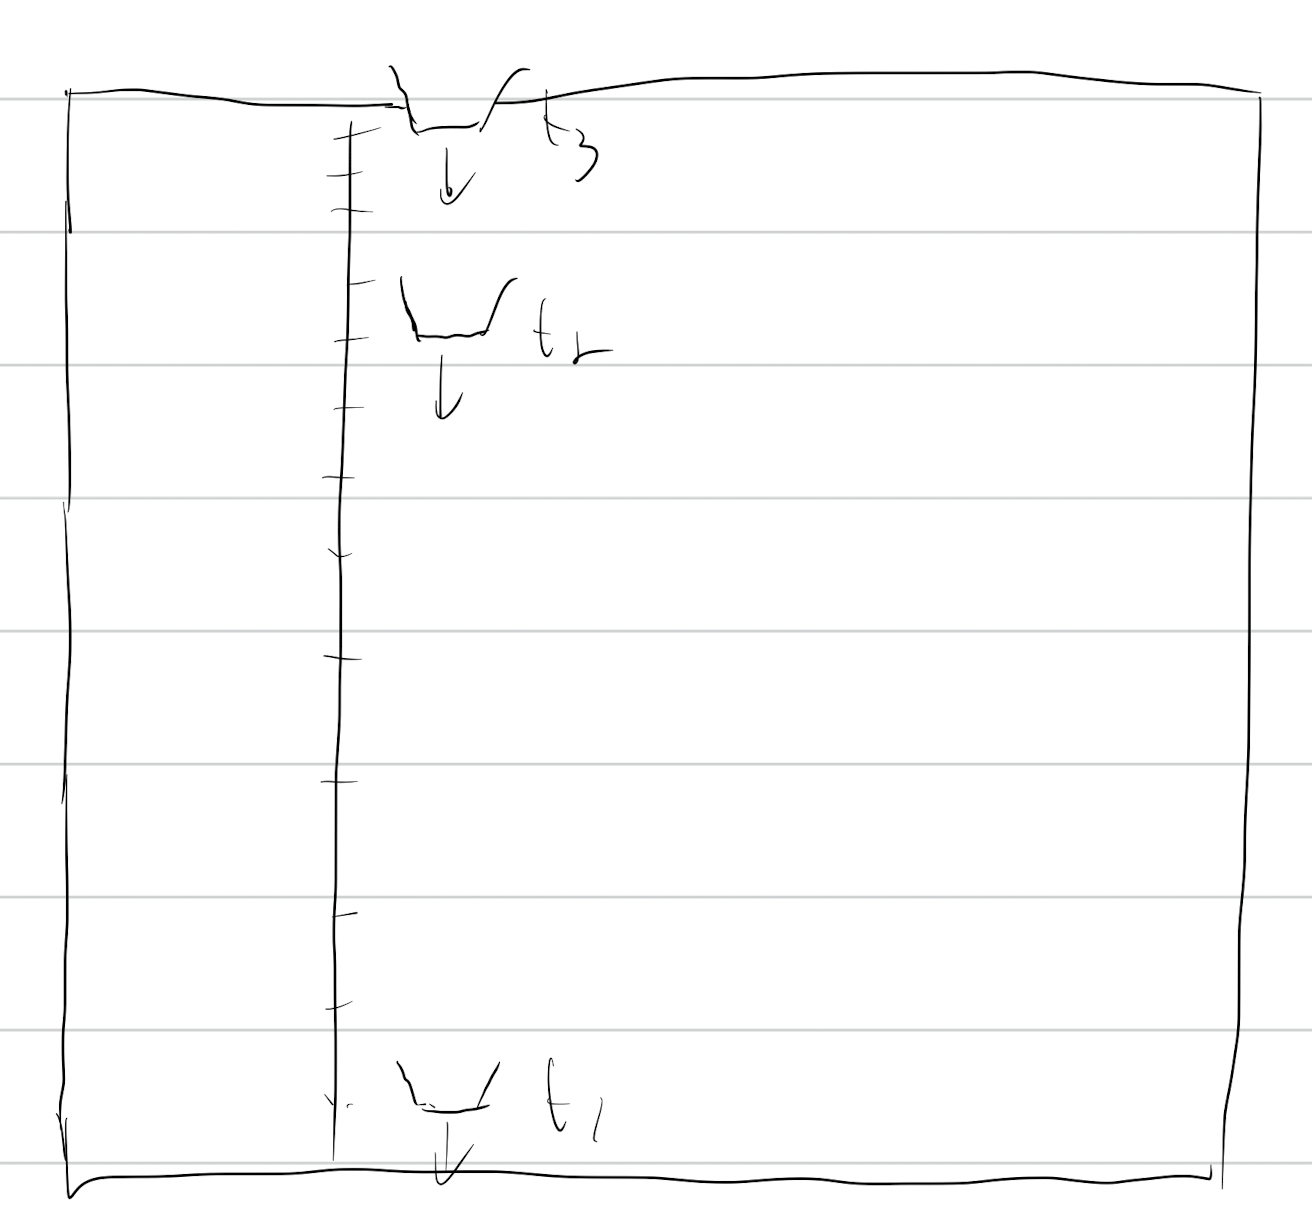
\includegraphics[width=10cm]{Lab6Image1_1}
\end{center}
\subsubsection*{Materials Necessary}
\begin{itemize}
	\item Coffee Filters
	\item Stopwatch
	\item Meter Stick (for measurement purposes)
	\item Wall
\end{itemize}
\subsubsection*{Measurements}
\begin{itemize}
	\item Height: $h$, in meters
	\item Time: $t$, in seconds
	\item Height error: $\delta h$, in meters
	\item Time error: $\delta t$, in seconds
\end{itemize}
\subsubsection*{Data Analysis}
The times on each of the measurements will be squared, and graphed on the $x$ axis with $h$ on the $y$ axis.
\begin{itemize}
	\item If the graph between $h$ and $t^2$ has a linear relationship (or close to one), then the tested idea is correct\textemdash namely that $h = \frac{1}{2} kt^2$ is correct.
	\item If the graph between $h$ and $t^2$ does not have a linear relationship, then the tested idea is incorrect.
\end{itemize}
\subsection*{Experiment 2}
\subsubsection*{Description}
The participants will position the motion sensor in ``person'' mode with the sonic side facing toward the floor, and position the coffee filter so that it falls similar to Experiment 1.
\subsubsection*{Sketch}
\begin{center}
	\includegraphics[width=10cm]{Lab6Image1_2}
\end{center}
\subsubsection*{Materials Necessary}
\begin{itemize}
	\item Coffee Filters
	\item Motion Sensor with associated software
	\item Stand to attach Motion Sensor to
\end{itemize}
\subsubsection*{Measurements}
\begin{itemize}
	\item Velocity: $v$, m/s
	\item Time: $t$, m/s
\end{itemize}
\subsubsection*{Data Analysis}
The graph of $v$ vs $t$ will be made with $t$ on the $x$ axis and $v$ on the $y$ axis.
\begin{itemize}
	\item If the graph between $v$ and $t$ is linear with a positive slope, then the tested idea is correct \textemdash namely, that $h$ and $t$ are related via $h = \frac{1}{2}kt^2$.
	\item If the graph between $v$ and $t$ is not linear with positive slope, but rather constant or some other value, then the tested prediction is wrong.
\end{itemize}
\pagebreak
\section*{Experiment 1}%
\subsection*{Part 1}%
10cm increments from $1.00$m to $2.00$m were measured out on a whiteboard, with a pushpin located on a bulletin board next to the whiteboard. The pushpin is attached about 20cm to the left of each of the increment marks as the experiment develops. The participant carries the coffee filter with their palm facing up and touches the pushpin with their fingers, Then, the participant drops the coffe filter by ``letting the bottom fall out'' by removing their arm in a lever action, starting the stopwatch at the same time. When the coffee filter hits the ground, the first participant stops the clock, and the second participant notes the time. This experimental technique was chosen as the square of the times corresponding to the heights should, in theory, display a linear graph starting from the origin passing through all the points if the predicted result is correct. A sketch of the experiment is shown below.
\begin{center}
	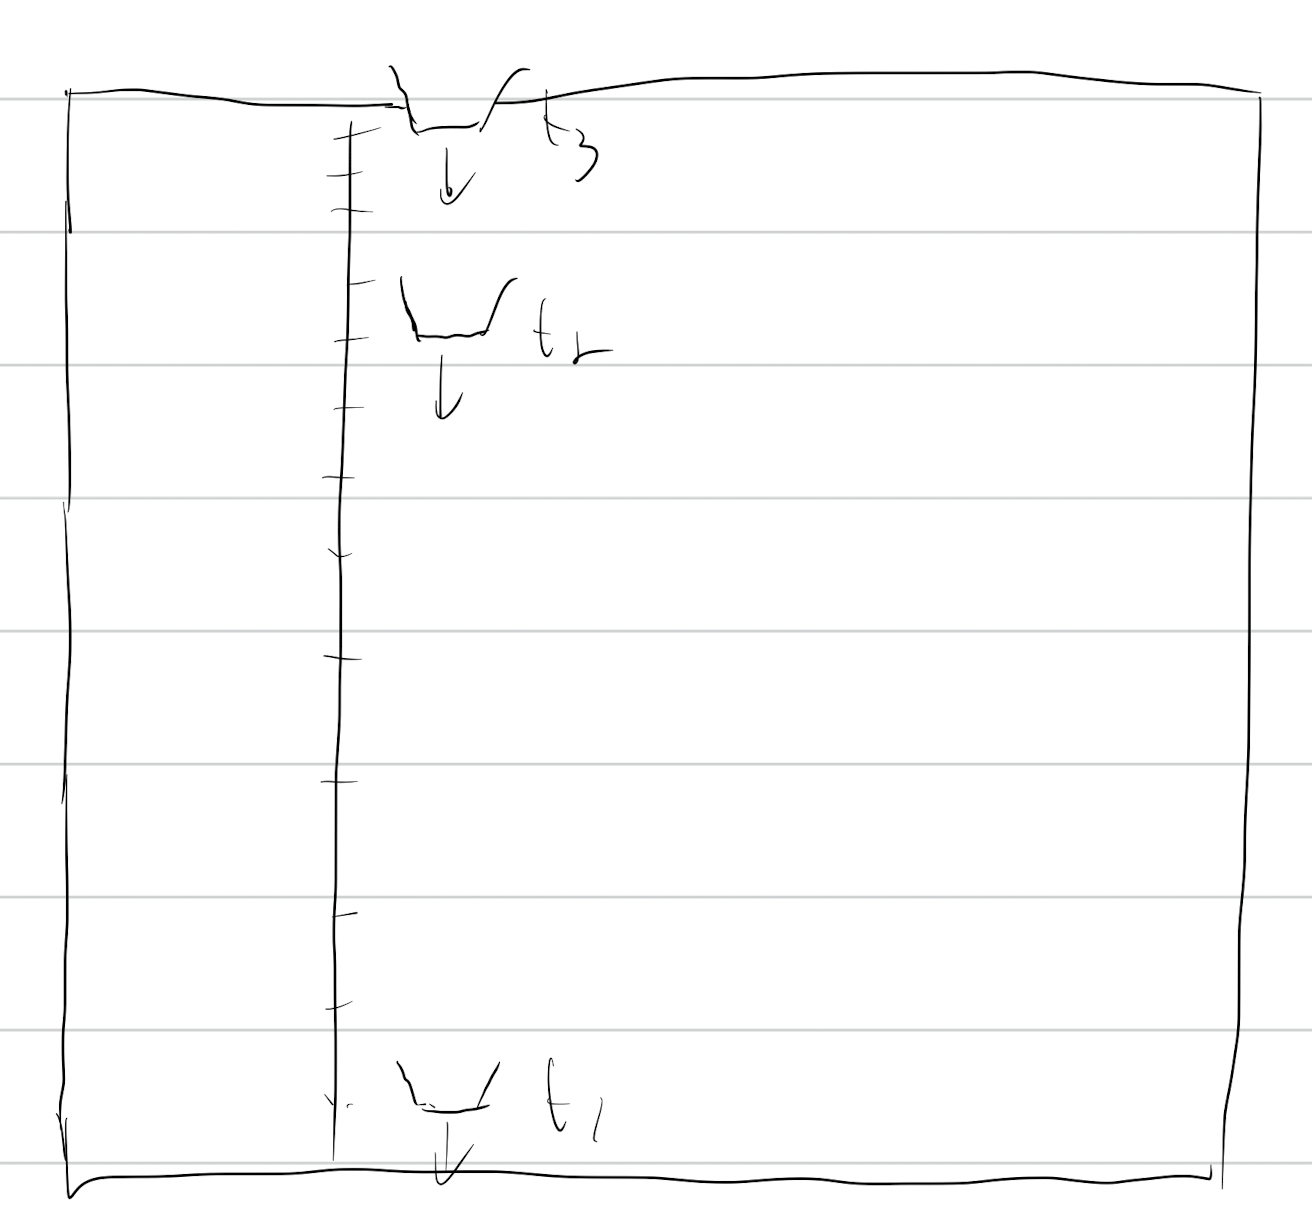
\includegraphics[width=10cm]{Lab6Image1_1}
\end{center}
\subsection*{Part 2}%
The predicted outcome would be that a graph of $t^2$ on the $x$ axis plotted against $h$ on the $y$ axis would yield a straight line, if it were consistent with the prediction that $h = \frac{1}{2}kt^2 $.
\subsection*{Part 3}%
We will make a graph with $t^2$ on the $x$ axis and $h$ on the $y$ axis, and attempt to find a curve of best fit which passes through the origin. If the curve is linear, then the prediction holds \textendash else, the prediction is thrown out.
\subsection*{Part 4}%
Our primary assumption is that the coffee filter falls in a straight line; if the coffee filter were to not fall in a straight line, the measured height $h$ would be lower than the actual distance the coffee filter fell, thus changing the graphed results.
\subsection*{Part 5}
The sources of experimental uncertainty include uncertainty in finding the time for the coffee filter to fall (mitigated by making the person who is the one letting the coffee filter fall also start the timer) and the measurement of height (mitigated by using a meter stick to mark on a whiteboard, which was then transferred over to the neighboring bulletin board by using a 15cm ruler). We assumed a time uncertainty of $0.3$s (similar to human reaction time) and a measurement uncertainty of $0.03$m, which is likely an overestimate.
\subsection*{Part 6}
The credibility of the method should be quite strong. We are using regressions and a fair number of data points to find if an empirical relation matches with a theoretical one in a manner that should be easily verifiable. However, the data that we collect will depend on fewer data points near the origin (as those will have high fractional uncertainty), increasing our dependence on the resulting regression curves to achieve our result.
\subsection*{Part 7}%
\begin{center}
	\renewcommand{\arraystretch}{1.5}
	\begin{tabular}{c|c|c|c|c}
		Height (m) & Trial 1 Time (s) & Trial 2 Time (s) & $t_{\textrm{avg}}$ & $t^2$ with error (s) \\
		\hline
		$h = 1.00 \pm 0.03$ & $t_1 = 0.89 \pm 0.3$ & $t_1 = 0.93\pm 0.3$& $t_1 = 0.91\pm 0.3$ & $t_1^2 = 0.8\pm 0.5$\\
		$h = 1.10 \pm 0.03$ & $t_2 = 1.03\pm 0.3$ & $t_2 = 1.05\pm 0.3$ & $t_2 = 1.04 \pm 0.3$	& $t_2^2 = 1.1\pm 0.6$\\
		$h = 1.20 \pm 0.03$ & $t_3 = 1.16 \pm 0.3$ & $t_3 = 1.11 \pm 0.3$ & $t_3 = 1.14\pm 0.3$ & $t_3^2 = 1.3 \pm 0.7$\\
		$h = 1.30 \pm 0.03$ & $t_4 = 1.36 \pm 0.3$ & $t_4 = 1.40 \pm 0.3$ & $t_4 = 1.38 \pm 0.3$ & $t_4^2 = 1.9 \pm 0.8$\\
		$h = 1.40 \pm 0.03$ & $t_5 = 1.46 \pm 0.3$ & $t_5 = 1.41 \pm 0.3$ & $t_5 = 1.44 \pm 0.3$ & $t_5^2 = 2.1 \pm 0.9$\\
		$h = 1.50 \pm 0.03$ & $t_6 = 1.47 \pm 0.3$ & $t_6 = 1.47 \pm 0.3$ & $t_6 = 1.47 \pm 0.3$ & $t_6^2 = 2.2 \pm 1.0$\\
		$h = 1.60 \pm 0.03$ & $t_7 = 1.54 \pm 0.3$ & $t_7 = 1.69 \pm 0.3$ & $t_7 = 1.62 \pm 0.3$ & $t_7^2 = 2.6 \pm 1.0$\\
		$h = 1.70 \pm 0.03$ & $t_8 = 1.81 \pm 0.3$ & $t_8 = 1.66 \pm 0.3$ & $t_8 = 1.74 \pm 0.3$ & $t_8^2 = 3.0 \pm 1.0$\\
		$h = 1.80 \pm 0.03$ & $t_9 = 1.90 \pm 0.3$ & $t_9 = 1.84 \pm 0.3$ & $t_9 = 1.87 \pm 0.3$ & $t_9^2 = 3.5 \pm 1.1$\\
		$h = 1.90 \pm 0.03$ & $t_{10} = 2.04\pm 0.3$ & $t_{10} = 1.90 \pm 0.3$ & $t_{10} = 1.97\pm 0.3$ & $t_{10}^2 = 3.8\pm 1.2$\\
		$h = 2.00 \pm 0.03$ & $t_{11} = 1.97\pm 0.3$ & $t_{11} = 2.00 \pm 0.3$ & $t_{11} = 1.99 \pm 0.3$ & $t_{11}^2 = 3.9\pm 1.2$
	\end{tabular}
\end{center}
\begin{center}
	\resizebox{12cm}{!}{
	\begin{tikzpicture}
		\begin{axis}[
			title={$t^2$ vs $h$},
			xlabel={$t^2$ (seconds$^2$)},
			ylabel={$h$ (meters)},
			xmin = 0, xmax = 5,
			ymin=-0.2, ymax = 2.5,
			xtick={0,1,2,3,4,5},
			ytick={0,0.5,1,1.5,2,2.5},
			xmajorgrids=true, ymajorgrids=true, grid style = dashed,
			]
			\addplot[only marks, mark = o, error bars/.cd, y dir = both, x dir = both, x explicit, y explicit] table[x index=0, x error index=1, y index=2, y error index=3]{images/Lab6Data1.dat};
		\end{axis}
	\end{tikzpicture}
	}
\end{center}
\begin{center}
	\resizebox{12cm}{!}{
		\begin{tikzpicture}
			\begin{axis}[
				title={$t^2$ vs $h$ with Linear Regression},
				xlabel={$t^2$ (seconds$^2$)},
				ylabel={$h$ (meters)},
				xmin = 0, xmax = 5,
				ymin=-0.2, ymax = 2.5,
				xtick={0,1,2,3,4,5},
				ytick={0,0.5,1,1.5,2,2.5},
				xmajorgrids=true, ymajorgrids=true, grid style = dashed,
				legend pos=south east,
			]
				\addplot[only marks, mark = o, error bars/.cd, y dir = both, x dir = both, x explicit, y explicit] table[x index=0, x error index=1, y index=2, y error index=3]{images/Lab6Data1.dat};
				\addlegendentry{\tiny Data}
				\addplot[color=blue,thin,domain=0:5,samples=100]{0.3*x+0.784};
				\addlegendentry{\tiny Linear Regression: $t^2 = 0.3h+0.784$}
			\end{axis}
		\end{tikzpicture}
	}
\end{center}
\begin{center}
	\resizebox{12cm}{!}{
		\begin{tikzpicture}
			\begin{axis}[
				title={$t^2$ vs $h$ with Power Series Regression},
				xlabel={$t^2$ (seconds$^2$)},
				ylabel={$h$ (meters)},
				xmin = 0, xmax = 5,
				ymin=-0.2, ymax = 2.5,
				xtick={0,1,2,3,4,5},
				ytick={0,0.5,1,1.5,2,2.5},
				xmajorgrids=true, ymajorgrids=true, grid style = dashed,
				legend pos=south east,
			]
				\addplot[only marks, mark = o, error bars/.cd, y dir = both, x dir = both, x explicit, y explicit] table[x index=0, x error index=1, y index=2, y error index=3]{images/Lab6Data1.dat};
				\addlegendentry{\tiny Data}
				\addplot[color=red,thin,domain=0:5,samples=100]{(1.06)*x^(0.43)};
				\addlegendentry{\tiny Power Series Regression: $t^2 = 1.06h^{0.43}$}
			\end{axis}
		\end{tikzpicture}
	}
\end{center}
\subsection*{Part 8}
Unlike the linear regression, the power series intersects the origin (as would be expected of any object falling any distance), meaning that it is more accurate than the linear regression. As such, the expected prediction that the data would resemble a linear function is \textbf{incorrect}.
\section*{Experiment 2}
\subsection*{Part 1}
One participant holds the acoustic motion sensor around shoulder level with one hand and rests a coffee filter on the palm of their other hand below the acoustic motion sensor. The second participant activates the motion sensor in the PASCO program, and the first participant lets the coffee filter fall in a manner similar to the first experiment. The resulting velocity vs. time graph in the PASCO program will be attached to the lab report.
\begin{center}
	\includegraphics[width=10cm]{images/Lab6Image1_2.png}
\end{center}
\subsection*{Part 2}
If the prediction holds, the resulting velocity vs. time graph should be linear with a consistent slope throughout the coffee filter falling. The slope of the graph will be equal to $k$ in the paper's prediction.
\subsection*{Part 3}
We used the motion sensor's graph of velocity vs. time to determine whether the coffee filter was falling with constant acceleration. If it was, then the slope of the graph of velocity vs. time would be equal to the constant within the prediction.
\subsection*{Part 4}
We assumed the coffee filter falls in a straight line when dropped, and that there was negligible air resistance.
\subsection*{Part 5}
Motion sensor not accurately capturing the coffee filter's fall: instead of dropping the coffee filter onto the motion sensor, we pointed the motion sensor down on top of the coffee filter. The motion sensor is close to the coffee filter, obviating the possibility of the motion sensor capturing something other than the coffee filter.
\subsection*{Part 6}
This is a quite credible system. The motion sensor is quite accurate in tracking the motion of the coffee filter. However, the software has to be connected to a computer at all times, so the coffee filter has a very short fall compared to what is possible measuring at each time. Additionally, the pathway the motion sensor detects has to be fully cleared, lest it picks up other objects.
\subsection*{Part 7}
\begin{center}
	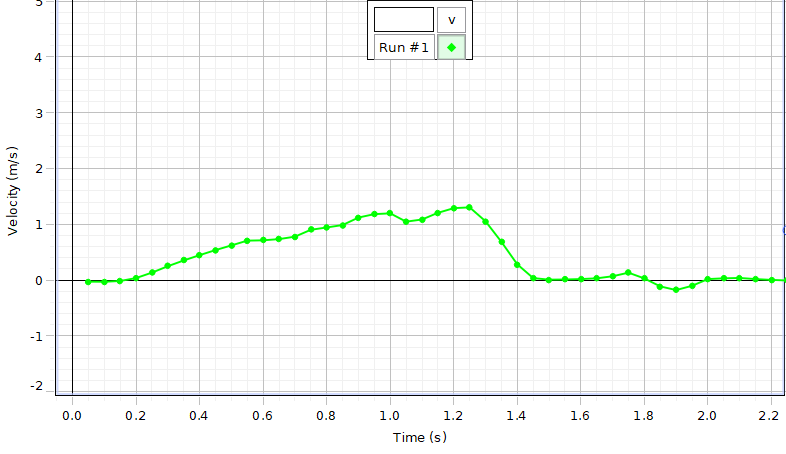
\includegraphics[width=10cm]{images/Lab6Image2_1.png}
\end{center}
\subsection*{Part 8}
In the early section of the graph, the coffee filter does follow a linear path as predicted. However, as time moves on, the coffee filter appears to take on constant velocity as the graph of velocity vs. time strays from the linear path.
\section*{Revisiting the Hypothesis}
Our new hypothesis is that early in the fall, the coffee filter takes on a distance function of $h = \frac{1}{2}kt^2$ for some acceleration $k$ that may or may not be equal to $g$. However, as time goes on, the coffee filter takes on the distance function of $h = vt$ for some terminal velocity $v$. \newline
\newline
The data satisfy this hypothesis in both steps. As seen in experiment 2, the coffee filter falls with linearly increasing velocity, implying constant acceleration throughout the early stages of the coffee filter's fall. Additionally, Experiment 1, which tested later stages of the coffee filter's fall, indicates a power series relation between $t^2$ and $h$, implying that $h$ increases linearly with $t$, or that $h = vt$ during later stages of the coffee filter's fall.
}\end{document}
